\documentclass[11pt]{article}
\usepackage[utf8]{inputenc}
\usepackage[T1]{fontenc}
\usepackage{fixltx2e}
\usepackage{graphicx}
\usepackage{grffile}
\usepackage{longtable}
\usepackage{wrapfig}
\usepackage{rotating}
\usepackage[normalem]{ulem}
\usepackage{amsmath}
\usepackage{textcomp}
\usepackage{amssymb}
\usepackage{capt-of}
\usepackage{hyperref}
\usepackage[english]{babel}
\author{Jay Dixit}
\date{\today}
\title{Emacs for Writers}
\hypersetup{
 pdfauthor={Jay Dixit},
 pdftitle={Emacs for Writers},
 pdfkeywords={},
 pdfsubject={},
 pdfcreator={Emacs 24.5.1 (Org mode 8.3.1)}, 
 pdflang={English}}
\begin{document}

\maketitle
\tableofcontents
\newpage


\section{Emacs for Writers\hfill{}\textsc{slide}}
\label{sec:orgheadline1}
\textbf{How I found my way to Emacs} 

Jay Dixit  \\
The New York Writers' Intensive \\
Twitter: \href{http://twitter.com/jaydixit}{@jaydixit}  \\
jay@jaydixit.com \\
newyorkwritersintensive.com \\

\section{My first computer\hfill{}\textsc{slide}}
\label{sec:orgheadline3}

\url{https://upload.wikimedia.org/wikipedia/commons/9/99/DEC_VT100_terminal.jpg} 

\subsubsection{Notes\hfill{}\textsc{notes}}
\label{sec:orgheadline2}
At work he had some kind of Vax Station\ldots{}
and at home we had a VT terminal 

But it wasn't mine. It belonged to the university.

\section{Modem\hfill{}\textsc{slide}}
\label{sec:orgheadline5}
\url{https://c2.staticflickr.com/4/3227/2979693877_c601ac432a.jpg} 

\subsubsection{Notes\hfill{}\textsc{notes}}
\label{sec:orgheadline4}
And our modem looked like this 

\section{VAX Terminal\hfill{}\textsc{slide}}
\label{sec:orgheadline7}
\includegraphics[width=.9\linewidth]{/Users/jay/Downloads/Screenshots/2015-09-14.png}
\subsubsection{Notes\hfill{}\textsc{notes}}
\label{sec:orgheadline6}

It was a black screen with yellow text, like this: 
Dear Dad.

How are you? I am fine.

How is Switzerland? I have been reading Isaac Asimov's Robot Dreams. It is depressing, and really makes you think. 

I have a game called the Hitchiker's Guide to the Galaxy. I have defeated the Bugblatter Beast, but I am having trouble getting the Babel fish. 

When are you coming home? I miss you. 

Love,
Sunjay

P.S. Tomorrow I present my Gifted project on Atlantis. 

\section{Dungeon (Zork)\hfill{}\textsc{slide}}
\label{sec:orgheadline8}
\url{http://xmedia.ex.ac.uk/wp/wordpress/wp-content/uploads/2014/10/zork.png} 

\section{My own computer\hfill{}\textsc{slide}}
\label{sec:orgheadline9}
\url{http://www.vectronicsappleworld.com/archives/vintage/images/0032/snap13.jpg} 

\section{Microsoft Word\hfill{}\textsc{slide}}
\label{sec:orgheadline10}
\url{http://computersandcomposition.candcblog.org/archives/v10/10_2_html/10_2_8_Boudreau1.gif} 

\section{Microsoft Word\hfill{}\textsc{slide}}
\label{sec:orgheadline11}
\url{http://i260.photobucket.com/albums/ii8/patheticcockroach/microsoft-word-sucks-write-without-.gif} 

\section{New Project\hfill{}\textsc{slide}}
\label{sec:orgheadline12}
\url{https://johntomsett.files.wordpress.com/2013/03/1984-opening-paragraph.jpg} 

\section{Googling\hfill{}\textsc{slide}}
\label{sec:orgheadline13}
\includegraphics[width=.9\linewidth]{/users/jay/Downloads/Screenshots/googling.png} 

\section{Workflowy\hfill{}\textsc{slide}}
\label{sec:orgheadline14}
\url{http://3.bp.blogspot.com/_oB6fkceAJrc/TSXTDtU_LiI/AAAAAAAABi8/gLOs_kICDZU/s1600/organize-goals-alt.png} 

\section{Scrivener\hfill{}\textsc{slide}}
\label{sec:orgheadline15}
\url{http://www.autostraddle.com/wp-content/uploads/2012/11/scrivener.jpg} 

\section{Scrivener\hfill{}\textsc{slide}}
\label{sec:orgheadline16}
\url{http://a5.mzstatic.com/us/r30/Purple/v4/fe/7b/16/fe7b1653-3165-7329-6ed8-60c10d4c4d5e/screen800x500.jpeg} 

\section{I needed a better solution\hfill{}\textsc{slide}}
\label{sec:orgheadline18}
\includegraphics[width=.9\linewidth]{/Users/jay/Downloads/Screenshots/DIY-mustard.png} 

\subsubsection{Notes\hfill{}\textsc{notes}}
\label{sec:orgheadline17}
So I did what I always do. Internet research.
\begin{itemize}
\item blenders
\item coffee grinders
\item ergonomic keyboards
\end{itemize}

\section{the original email\hfill{}\textsc{slide}}
\label{sec:orgheadline20}
\url{http://i.imgur.com/263uwKv.jpg} 

\subsubsection{Notes\hfill{}\textsc{notes}}
\label{sec:orgheadline19}
Is there an app that displays keyboard-editable hierarchical structure in the left pane and text editing/word processing in the right pane?

I'm looking for a Mac or web-based app that will allow me to create and modify hierarchical structure (in the form of multi-level bulleted lists) in the left pane and do text editing/word processing in the right pane.

I wish I could combine Workflowy and Scrivener into one tool.

The good thing about Scrivener: It displays the hierarchical structure of my document in the left pane (with headers, subheaders, subsubheaders) and displays a text editor/word processor in the right pane.

The problem with Scrivener: Creating new sections, moving sections around, nesting one section beneath another, etc is cumbersome. Every time you want a new level of the hierarchy, you have to choose ``new text,'' name it, and use the trackpad (not the keyboard) to drag it to where you want it in document folder structure. Blech.

The good thing about Workflowy: Creating and modifying the hierarchical structure is so easy. You create a new list item simply by hitting enter, promote by hitting tab, demote by hitting shift-tab, and move list items around easily using the keyboard. The problem with Workflowy: no text editor pane.

What I want is a tool that's like Workflowy in the left pane---quick keyboard-based creating and modifying of hierarchical structure---but with a text editor/word processor in the right pane.

With the tool I envision, for each bulleted list item in the left-pane hierarchy, I could enter right-pane text. At the end, like Scrivener, the tool would ``compile'' a Word document, excluding the hierarchy of headers and subheaders and including only the right-pane text.

I can hack a solution to this with Workflowy by just entering body text below various list items in the structural hierarchy and adding a \#bodytext tag for each paragraph of prose, then running a search for \#bodytext and exporting only the paragraphs that appear thus tagged. But it would be more far more useful to have a split-screen navigation so that I could see the body text in a separate pane from the hierarchical structure.

I looked at Omni Outliner, and with that tool, I do not seem to be able to select and export by hierarchical level, so I don't think I could isolate the body text.

Does such a tool exist? What solutions would you suggest? Thanks! 

Jay Dixit

\section{Re: outlining in the left pane, text in the right?\hfill{}\textsc{slide}}
\label{sec:orgheadline22}
\begin{quote}
From: Lucas 
In the past, I used Mori for this sort of outlining and found it well suited. Both folders and notes can be hierarchically organized, and you can used the app's ``Widescreen Layout'' to get to the sort of set-up you're looking for. There are export options, but I don't know know whether they would fit your needs. Development has been scarce and erratic in recent years, but you can try Mori for free. 
\end{quote}

\subsubsection{Notes\hfill{}\textsc{notes}}
\label{sec:orgheadline21}
In the past, I used Mori for this sort of outlining and found it well suited. Both folders and notes can be hierarchically organized, and you can used the app's ``Widescreen Layout'' to get to the sort of set-up you're looking for. There are export options, but I don't know know whether they would fit your needs. Development has been scarce and erratic in recent years, but you can try Mori for free. 

\section{Re: outlining in the left pane, text in the right?\hfill{}\textsc{slide}}
\label{sec:orgheadline24}
\begin{quote}
From: Stephen Zoll 
OP is asking about something that's hard to find in modern ``outlining'' applications, even harder on Macs. Most Mac apps of this sort (DevonThink, Together) rely on a folder structure to build hierarchy. Few allow you to nest one note under another. In most cases, shifting back and forth between the ``tree'' and the editor is awkward. Those apps with strong editor panes are not set up to make the tree pane easy to edit and organize. It's odd that this seems so difficult to code, because it seems like a perfectly legitimate request: An application where it's easy to move between the editor and the outline, and where the outline is easy to edit and restructure using the keyboard. I agree with MadAboutDana that Tree is a good option to try, though the notes are inline and not in a separate, right-hand pane as the original poster requests. Steve Z. 
\end{quote}

\subsubsection{Notes\hfill{}\textsc{notes}}
\label{sec:orgheadline23}
OP is asking about something that's hard to find in modern ``outlining'' applications, even harder on Macs. Most Mac apps of this sort (DevonThink, Together) rely on a folder structure to build hierarchy. Few allow you to nest one note under another. In most cases, shifting back and forth between the ``tree'' and the editor is awkward. Those apps with strong editor panes are not set up to make the tree pane easy to edit and organize. It's odd that this seems so difficult to code, because it seems like a perfectly legitimate request: An application where it's easy to move between the editor and the outline, and where the outline is easy to edit and restructure using the keyboard. I agree with MadAboutDana that Tree is a good option to try, though the notes are inline and not in a separate, right-hand pane as the original poster requests. Steve Z. 


\section{Re: outlining in the left pane, text in the right?\hfill{}\textsc{slide}}
\label{sec:orgheadline26}
\begin{quote}
From: JBfrom. Posted by Nov 19, 2011 at 01:07 PM You can do this in Emacs Org-Mode by using indirect buffer, vertical split screen, and visibility cycling. Everything is handled via hotkeys. It's available for Mac. I frequently work in this mode for longer documents. 
\end{quote}

\subsubsection{Notes\hfill{}\textsc{notes}}
\label{sec:orgheadline25}
From: JBfrom. Posted by Nov 19, 2011 at 01:07 PM You can do this in Emacs Org-Mode by using indirect buffer, vertical split screen, and visibility cycling. Everything is handled via hotkeys. It's available for Mac. I frequently work in this mode for longer documents. 


\section{Re: outlining in the left pane, text in the right?\hfill{}\textsc{slide}}
\label{sec:orgheadline28}
\begin{quote}
From: Jay Dixit 
JBfrom, emacs org-mode sounds like a great solution. I'm intrigued. It also looks a little complicated, but if it indeed does exactly what I'm describing, then I'm willing to take on a learning curve. I've downloaded emacs and org-mode. Can you describe how to set it up to do this, or direct me to a resource that will? 
\end{quote}
\subsubsection{Notes\hfill{}\textsc{notes}}
\label{sec:orgheadline27}
From: Jay Dixit 
JBfrom, emacs org-mode sounds like a great solution. I'm intrigued. It also looks a little complicated, but if it indeed does exactly what I'm describing, then I'm willing to take on a learning curve. I've downloaded emacs and org-mode. Can you describe how to set it up to do this, or direct me to a resource that will? 


\section{Taking the first step\hfill{}\textsc{slide}}
\label{sec:orgheadline30}
\begin{quote}
Hey Joseph, 
Thanks for the tip about emacs org mode. It looks a little scary but I'm ready to try it out. 
I'm trying to get started and I've gotten stuck. Wondering if you can help me.
I've installed emacs and ergoemacs on my Mac. Now I need to install org mode. 
I downloaded org mode and I'm trying to install it. The documentation simply says:
To install org­mode, edit the Makefile, type `make', then `make install'.
To create the PDF and HTML documentation files, type `make doc'. 
But where am I supposed to type these things? In Terminal? Do I somehow type them in emacs itself? If so, how do I get a prompt in emacs so I can type commands? 
\end{quote}

\subsubsection{Notes\hfill{}\textsc{notes}}
\label{sec:orgheadline29}
Hey Joseph,

Thanks for the tip about emacs org mode. It looks a little scary but I'm ready to try it out.

I'm trying to get started and I've gotten stuck. Wondering if you can help me.
I've installed emacs and ergoemacs on my Mac. Now I need to install org mode.

I downloaded org mode and I'm trying to install it. The documentation simply says:
To install org­mode, edit the Makefile, type `make', then `make install'.
To create the PDF and HTML documentation files, type `make doc'.

But where am I supposed to type these things? In Terminal? Do I somehow type them in emacs itself? If so, how do I get a prompt in emacs so I can type commands? 

\section{n00b\hfill{}\textsc{slide}}
\label{sec:orgheadline32}

\includegraphics[width=.9\linewidth]{/users/jay/Dropbox/presentations/emacs-presentation-slideshow/img/noob.jpg} 

\subsubsection{Notes\hfill{}\textsc{notes}}
\label{sec:orgheadline31}
I was definitely one of these guys\ldots{} Hey everybody had to start somewhere. 

\section{But\ldots{} I figured it out\hfill{}\textsc{slide}}
\label{sec:orgheadline33}
\includegraphics[width=.9\linewidth]{/Users/jay/Dropbox/writing/book/book-images/Screen-Shot-2013-03-06-at-7.29.29pm.png} 

\section{org-mode to write a book\hfill{}\textsc{slide}}
\label{sec:orgheadline34}
\includegraphics[width=.9\linewidth]{/Users/jay/Dropbox/writing/book/book-images/Screen-Shot-2013-05-31-at-1.39.52-AM.png} 

\section{commenting my prose\hfill{}\textsc{slide}}
\label{sec:orgheadline35}
\includegraphics[width=.9\linewidth]{/Users/jay/Dropbox/writing/book/book-images/Screen-Shot-2013-05-31-at-3.18.52-AM.png} 


\section{I still don't really know what I'm doing\hfill{}\textsc{slide}}
\label{sec:orgheadline36}

\includegraphics[width=.9\linewidth]{/users/jay/Dropbox/presentations/emacs-presentation-slideshow/img/code_quality-self-taught.png} 

\section{The Emacs Learning Curve\hfill{}\textsc{slide}}
\label{sec:orgheadline38}
\url{http://farm4.staticflickr.com/3109/3251176498_c3485a55fb.jpg} 

\subsubsection{Notes\hfill{}\textsc{notes}}
\label{sec:orgheadline37}
But my favorite is a blog post: learn Emacs in 10 years.
StackExchange
why I'm here 

\section{But at least I'm in good company\hfill{}\textsc{slide}}
\label{sec:orgheadline39}

\includegraphics[width=.9\linewidth]{/Users/jay/Dropbox/presentations/emacs-presentation-slideshow/img/George-RR-Martin.png} 

\section{Neal Stephenson\hfill{}\textsc{slide}}
\label{sec:orgheadline40}
\url{http://www.nealstephenson.com/assets/gallery/3/113.jpg} 

\section{Neil Stephenson\hfill{}\textsc{slide}}
\label{sec:orgheadline42}
\begin{quote}
The engineer-hours that, in the case of Microsoft Word, were devoted to features like mail merge, and the ability to embed feature-length motion pictures in corporate memoranda, were, in the case of emacs, focused with maniacal intensity on the deceptively simple-seeming problem of editing text. If you are a professional writer---i.e., if someone else is getting paid to worry about how your words are formatted and printed--emacs outshines all other editing software in approximately the same way that the noonday sun does the stars. It is not just bigger and brighter; it simply makes everything else vanish.
\end{quote}

\subsubsection{Notes\hfill{}\textsc{notes}}
\label{sec:orgheadline41}
The engineer-hours that, in the case of Microsoft Word, were devoted to features like mail merge, and the ability to embed feature-length motion pictures in corporate memoranda, were, in the case of emacs, focused with maniacal intensity on the deceptively simple-seeming problem of editing text. If you are a professional writer---i.e., if someone else is getting paid to worry about how your words are formatted and printed--emacs outshines all other editing software in approximately the same way that the noonday sun does the stars. It is not just bigger and brighter; it simply makes everything else vanish. 

\section{WordStar\hfill{}\textsc{slide}}
\label{sec:orgheadline43}

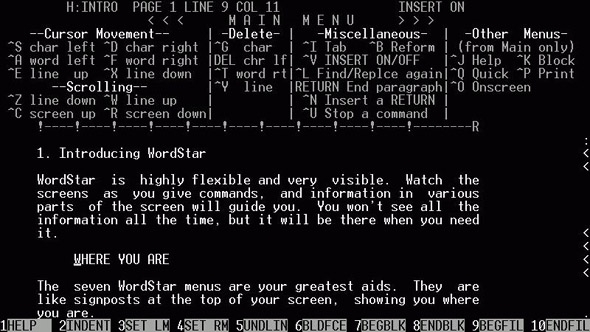
\includegraphics[width=.9\linewidth]{/Users/jay/Dropbox/presentations/emacs-presentation-slideshow/img/wordstar.jpg} 

\section{George R.R. Martin\hfill{}\textsc{slide}}
\label{sec:orgheadline44}

\includegraphics[width=.9\linewidth]{/Users/jay/Dropbox/presentations/emacs-presentation-slideshow/img/George-RR-Martin.png} 

\section{Richard Stallman\hfill{}\textsc{slide}}
\label{sec:orgheadline45}

\includegraphics[width=.9\linewidth]{/Users/jay/Dropbox/presentations/emacs-presentation-slideshow/img/Richard-Stallman.jpg} 

\section{The End\hfill{}\textsc{slide}}
\label{sec:orgheadline46}


\section{Org-HTML-Slideshow\hfill{}\textsc{slide}}
\label{sec:orgheadline59}

Make slides from Emacs Org-Mode!

\subsection{Making Slides\hfill{}\textsc{slide}}
\label{sec:orgheadline47}

Org-Mode headlines with the :slide: tag will become slides.

\subsection{Headlines Don't Have to be Slides}
\label{sec:orgheadline48}

This section doesn't have a :slide: tag, so it will \textbf{not} become a slide, although it is still part of the exported HTML document.

\subsection{Use \textbf{Lists} For \textit{Bullets}\hfill{}\textsc{slide}}
\label{sec:orgheadline49}

\begin{itemize}
\item Use Org-Mode lists for bullet points
\item You can make nested bullet lists
\begin{itemize}
\item With sub-lists
\item Like this
\end{itemize}
\end{itemize}

\subsection{Or Low-Level Headings\hfill{}\textsc{slide}}
\label{sec:orgheadline56}

\begin{enumerate}
\item By default
\label{sec:orgheadline53}
\begin{enumerate}
\item Org-Mode headings below level 3
\label{sec:orgheadline52}
\begin{enumerate}
\item Become bullets
\label{sec:orgheadline50}
\item Meaning they \textbf{cannot} be slides
\label{sec:orgheadline51}
\end{enumerate}
\end{enumerate}
\item This is configurable
\label{sec:orgheadline55}
\begin{enumerate}
\item See \href{http://orgmode.org/manual/Export-options.html}{Export Options in the Org-Mode manual}
\label{sec:orgheadline54}
\end{enumerate}
\end{enumerate}

\subsection{Slides Can Be Nested\hfill{}\textsc{slide}}
\label{sec:orgheadline58}

You can use the structure of the Org-Mode document to group your slides.

For example, this slide is a \textbf{level-2} Org-Mode heading.

\subsubsection{Slide Headings Can Be Nested\hfill{}\textsc{slide}}
\label{sec:orgheadline57}

This slide is a \textbf{level-3} Org-Mode heading, inside the previous one.

\section{Presenter Notes\hfill{}\textsc{slide}}
\label{sec:orgheadline62}

\begin{itemize}
\item Slides can have presenter notes
\item Add a sub-heading with the :notes: tag
\end{itemize}

\subsection{A Slide with Notes\hfill{}\textsc{slide}}
\label{sec:orgheadline61}

\begin{itemize}
\item This slide has notes
\item Notes are only visible to presenter
\end{itemize}

\subsubsection{Notes\hfill{}\textsc{notes}}
\label{sec:orgheadline60}

\begin{itemize}
\item Presenter notes for this slide
\item Not displayed as part of the slide
\item Displayed in Presenter Preview window
\item Only one :notes: section per slide allowed
\end{itemize}

\section{Source Code\hfill{}\textsc{slide}}
\label{sec:orgheadline65}

Use begin_/Users/jay/Dropbox/github/org-html-slideshow/src/end_src blocks to include source code.

\begin{verbatim}
  (defn example []
    (println "This is sample source code."))
\end{verbatim}

\subsection{Syntax Highlighting\hfill{}\textsc{slide}}
\label{sec:orgheadline63}

\begin{itemize}
\item Org-Mode HTML export uses \href{http://www.emacswiki.org/emacs/Htmlize}{htmlize.el}
\item Code in exported HTML will match your current Emacs theme
\begin{itemize}
\item Choose a theme that looks good on a projector!
\end{itemize}
\end{itemize}

\subsection{Syntax Highlighting with CSS Classes\hfill{}\textsc{slide}}
\label{sec:orgheadline64}

\begin{itemize}
\item Set the Emacs variable 
\begin{itemize}
\item org-export-htmlize-output-type
\item to the symbol css
\item (Does not work as a buffer-local variable)
\end{itemize}
\item Htmlize.el will add SPAN tags with CSS classes
\begin{itemize}
\item Named for each font face, e.g. org-comment
\end{itemize}
\item Examine HTML output to see class names
\item Add CSS styles to set colors
\end{itemize}

\section{Images\hfill{}\textsc{slide}}
\label{sec:orgheadline67}

\begin{itemize}
\item Slides can contain images
\begin{itemize}
\item Any file type a browser can display
\end{itemize}
\item See also these Emacs variables:
\begin{itemize}
\item org-export-html-inline-images
\item org-export-html-inline-image-extensions
\begin{itemize}
\item Controls which file types get exported
\end{itemize}
\end{itemize}
\item See \href{http://orgmode.org/manual/Images-in-HTML-export.html}{Images in HTML Export in the Org-Mode manual}.
\end{itemize}

\subsection{Slide with Image\hfill{}\textsc{slide}}
\label{sec:orgheadline66}

Make a file: link with the path to the image and no link text.

\includegraphics[width=.9\linewidth]{img/Jesus_paintingnew_293150090.jpeg} 

This example image is public-domain \href{http://openclipart.org/detail/165554/geodesic_dome-by-yoderj}{clip art by Josiah / yoderj}.

\section{Styling\hfill{}\textsc{slide}}
\label{sec:orgheadline69}

\begin{itemize}
\item Use CSS styles to control appearance of slides
\item Extra tags on a slide become extra CSS classes on its HTML
\end{itemize}

\subsection{Org-Mode Tag as CSS Class\hfill{}\textsc{slide:blue\_background}}
\label{sec:orgheadline68}

\begin{itemize}
\item This slide has the :blue_background: tag
\begin{itemize}
\item Which is a class defined in projection.css
\end{itemize}
\item Make up your own tags
\begin{itemize}
\item Add them to the CSS file
\end{itemize}
\end{itemize}

\section{Placing Stylesheets/JavaScript\hfill{}\textsc{slide}}
\label{sec:orgheadline72}

Include the stylesheets and JavaScript at the \textbf{bottom} of your Org-Mode file.

They must go at the bottom because the Google Closure Library does not support an on-DOM-ready event. See the \href{http://groups.google.com/group/closure-library-discuss/browse_thread/thread/1beecbb5d6afcb41/075c536259653946}{Closure mailing list discussion} for an explanation.

\subsection{Warning About Hidden Headlines\hfill{}\textsc{slide}}
\label{sec:orgheadline70}

Stylesheets and JavaScript will \textbf{not} be loaded if the \textbf{last} headline in your Org-Mode file is hidden by any of:

\begin{itemize}
\item COMMENT at the start of the heading
\item #+COMMENT at the start of the line
\item :noexport: tag, or missing :export: tag
\end{itemize}

See \href{http://orgmode.org/manual/Comment-lines.html}{Comment lines} and \href{http://orgmode.org/manual/Selective-export.html}{Selective export} in the Org-Mode manual for details.

org-html-head-include-scripts

\subsection{The End\hfill{}\textsc{slide}}
\label{sec:orgheadline71}

Sometimes it's safest to add an ``empty'' heading at the end of your document to make sure the stylesheets and JavaScript are included.
\end{document}